
\documentclass[12pt]{article}
\usepackage{amssymb, amsmath, amsthm, amsfonts}
\usepackage{epic}
\usepackage{eepic}
%\usepackage{hyperref}
\usepackage{listings}
\usepackage{float}
\usepackage[caption = false]{subfig}
\usepackage{graphicx}
\usepackage{fancyhdr}
\usepackage{color}
\usepackage{enumitem}
\usepackage[letterpaper, margin=1in]{geometry}
\usepackage{mathrsfs}
\usepackage{cleveref}

\newcommand{\C}{\mathbf{C}}
\newcommand{\R}{\mathbf{R}}
\newcommand{\Q}{\mathbf{Q}}
\newcommand{\Z}{\mathbf{Z}}
\newcommand{\N}{\mathbf{N}}
\newcommand{\E}{\mathbf{E}}
\newcommand{\B}{\mathbf{B}}
\newcommand{\F}{\mathbf{F}}
\newcommand{\U}{\mathbf{U}}
\newcommand{\V}{\mathbf{V}}
\newcommand{\J}{\mathbf{J}}
\newcommand{\x}{\mathbf{x}}
\newcommand{\y}{\mathbf{y}}
\newcommand{\z}{\mathbf{z}}
\newcommand{\Ib}{\mathbb{I}}
\newcommand{\Sb}{\mathbf{S}}
\newcommand{\Cs}{\mathscr{C}}
\newcommand{\As}{\mathscr{A}}
\newcommand{\xb}{\mathbf{x}}
\newcommand{\I}{\textnormal{\textbf{I}}}
\newcommand{\Id}{\dot{\textnormal{\textbf{I}}}}
\newcommand{\Top}{\textnormal{\textbf{Top}}}
\newcommand{\hTop}{\textnormal{\textbf{hTop}}}
\newcommand{\Groups}{\textnormal{\textbf{Groups}}}
\newcommand{\Set}{\textnormal{\textbf{Set}}}
\newcommand{\Xib}{\mathbf{\Xi}}
\newcommand{\Sym}{\text{Sym}}
\newcommand{\prid}[1]{\langle #1 \rangle}
\newcommand{\apoly}[1]{a_{#1} + a_{#1}x+ a_{#1}x^2 + \cdots + a_{#1}x^n}
\newcommand{\dist}{\textnormal{dist}}
\newcommand{\ti}[1]{\textit{#1}}
\newcommand{\tb}[1]{\textnormal{\textbf{#1}}}
\newcommand{\es}{\emptyset}
\newcommand{\sst}{\subset}
\newcommand{\ssteq}{\subseteq}
\newcommand{\func}[3]{#1: #2 \to #3}
\newcommand{\inte}[1]{\textnormal{int}(#1)}
\newcommand{\bdr}[1]{\textnormal{bdry}(#1)}
\newcommand{\ifff}{if and only if }
\newcommand{\st}{such that }
\newcommand{\wrt}{with respect to }
\newcommand{\tspace}[1]{\text{T}_#1}
\newcommand{\mathdash}{\hbox{-}}
\newcommand{\diam}[1]{\textnormal{diam}(#1)}
\newcommand{\setst}{\hspace{1mm} | \hspace{1mm} }
\newcommand{\supp}{\textnormal{support}}
\newcommand{\clos}{\textnormal{closure}}
\newcommand{\rel}{\textnormal{rel }}
\newcommand{\Hom}{\textnormal{Hom}}
\newcommand{\obj}{\textnormal{obj}}
\newcommand{\varlisto}[2]{#1_1,#1_2,\ldots,#1_{#2}}
\newcommand{\varlistz}[2]{#1_0,#1_1,\ldots,#1_{#2}}
\newcommand{\finv}[2]{#1^{-1}(#2)}
\newcommand{\disu}{\rotatebox[origin=c]{90}{$\models$}}
\newcommand{\rank}{\textnormal{rank }}
\newcommand{\card}{\textnormal{card }}
\newcommand{\im}{\textnormal{im }}
\newcommand{\cls}{\textnormal{cls }}
\newcommand{\rev}{\textnormal{rev }}
\newcommand{\defeq}{\mathrel{\stackrel{\makebox[0pt]{\mbox{\normalfont\tiny def}}}{=}}}
\newcommand{\Err}{\textnormal{Err}}
\newcommand{\Var}{\textnormal{Var}}
\newcommand{\Ev}{\textnormal{E}}
\newcommand{\pii}[1]{\exp(\beta_{#1}^Tx_i)}
\newcommand{\spii}[1]{\sum_{#1 = 1}^C\exp(\beta_{#1}^Tx_i)}
\newcommand{\spij}[1]{\sum_{#1 = 1}^C\exp(\beta_{#1}^Tx_{i,j})}
\newcommand{\dpp}{\partial}

\renewcommand{\epsilon}{\varepsilon}



\newtheorem{theorem}{Theorem}[section]
\newtheorem{corollary}[theorem]{Corollary}
\newtheorem{proposition}{Proposition}[theorem]
\newtheorem{lemma}[theorem]{Lemma}
\theoremstyle{definition}
\newtheorem*{solution*}{Solution}
\newtheorem*{definition}{Definition}
\newtheorem*{remark}{Remark}
\newtheorem*{remarks}{Remarks}


\renewcommand\qedsymbol{$\blacksquare$}

\author{Luke Meszar}
\date{September 15th, 2017}
\title{CSCI 5622 Homework 1}

\begin{document}
	\thispagestyle{empty}
	
	% --- Header Box --- %
	\newlength{\boxlength}\setlength{\boxlength}{\textwidth}
	\addtolength{\boxlength}{-4mm}
	
	\begin{center}\framebox{\parbox{\boxlength}{\bf
				Machine Learning \hfill Homework 4\\
				CSCI 5622 Fall 2017 \hfill Due Time Nov 10, 2017\\
				Name: Luke Meszar \hfill CU identitykey: lume0018
		}}
	\end{center}
	\section{Support Vector Machines (50 pts)}																																									
	\begin{solution*}\leavevmode
		\begin{enumerate}[label=\arabic*.,font=\upshape]
			\setcounter{enumi}{2}
			\item \textit{ Comment on classification performance for each model for optimal parameters by either
				testing on a hold-out set or performing cross-validation.}
			
				My strategy for grid search  was to first do a grid search for the optimal parameters for each of the three kernels. In each case, I started by testing over a large range of values for the parameters. Then, after seeing which one performed the best, I searched over a smaller range centered around this value. This was done to save on total computation time. I  Then, using the best parameters found in these three steps, I did a final grid search over all three kernels to find the outright beset model. For all grid searches, I used 3 fold cross-validation on the training data. 
				
				For the linear kernel, I searched for over the values $\{0.05,0.1,0.2,0.3\}$ for the penalty parameters $C$. I found that the optimal value for $C$ was 0.2 with a test accuracy of 0.972. 
				
				For the polynomial kernel, I searched for $C$ over the values $\{1,100,200,300,400,500, 600,700,800,900,1000,2000,3000,4000,5000,6000,7000,8000,9000\}$ and I searched the degree over the values $\{1,2,3\}$. I found the optimal parameters were $C = 5000$ with a degree of 2. This model scored a test accuracy of 0.989. 
				
				For the rbf kernel, I searched for $C$ over the values $\{1,10,20,30,40,50,75,100\}$ and I search for $\gamma$ over the values $\{.001,0.01,0.1\}$. I found the optimal value parameters were $C = 20$ and $\gamma = 0.01$. This model achieved a test accuracy of 0.991.
				
				Finally, to search for the best parameters overall, I had a parameters grid that looked like.
				
				\begin{align*}
				[\{'C':[0.05,0.1,0.2,0.15],'kernel':['linear']\},
				\\\{'C': [1000,2000,3000,4000,5000],
				'kernel':['poly'],'degree':[2,3,4]\},\\\{'C': [10,20,30,40,50],'kernel':['rbf'],'gamma':[0.001,0.01,0.1]\}]
				\end{align*}
				
				Here, I found the best parameters were an rbf kernel with $C = 20$ and $\gamma = 0.01$. Again, this model achieved a test accuracy of 0.991.
	
			\item \textit{ Give examples (in picture form) of support vectors from each class when using a polynomial
				kernel.}
			
			Below are four random examples of support vectors from the SVM using an rfb kernel with $C = 20$ and $\gamma = 0.01$. We can see, especially in Figure \ref{sfig:almost4-1} and Figure \ref{sfig:almost4-2}, that these two examples that are labeled as 9's look pretty similar to 4's. It makes sense that images corresponding to support vectors would look like the opposite class since support vectors lie closest to the hyperplane separating the two classes. 
			
			\begin{figure}[H]
				\subfloat[]{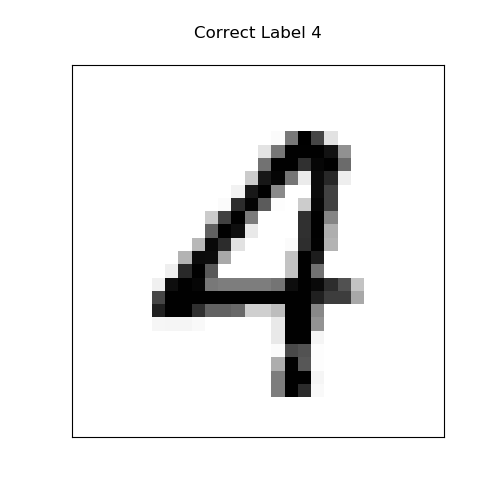
\includegraphics[width = 1.5in,height=1.5in]{support_vector0}}
				\subfloat[\label{sfig:almost4-1}]{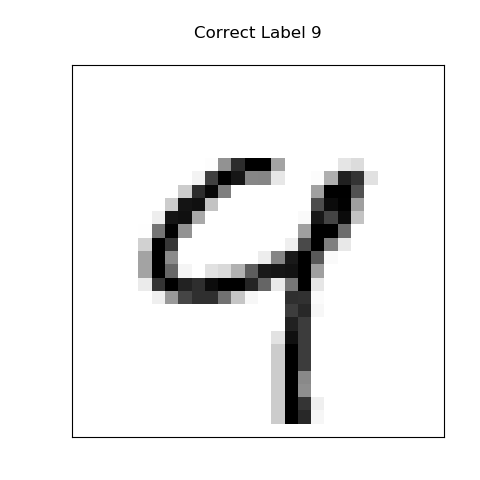
\includegraphics[width = 1.5in,height=1.5in]{support_vector1}}\\
				\subfloat[\label{sfig:almost4-2}]{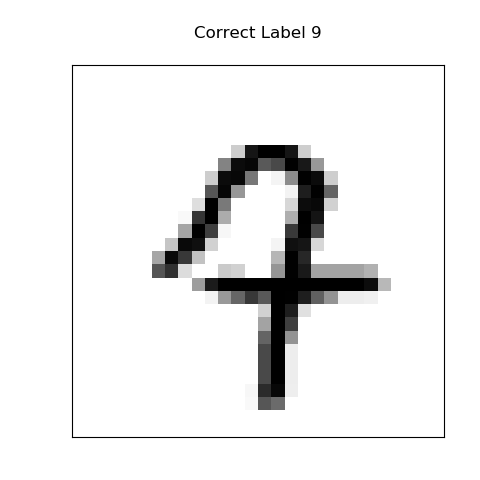
\includegraphics[width = 1.5in,height=1.5in]{support_vector2}}
				\subfloat[]{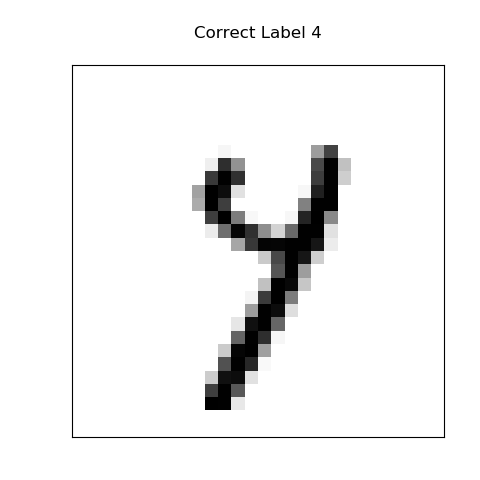
\includegraphics[width = 1.5in,height=1.5in]{support_vector_1}} \\
				\caption{Support vectors for an SVM using an rfb kernel with $C = 20$ and $\gamma = 0.01$}
				\label{}
			\end{figure}
			
		\end{enumerate}
	\end{solution*}
	\section{Learnability (25 pts)}
	\begin{solution*}
		\textit{Consider the class C of concepts defined by triangles with distinct vertices of the form (i,j) where
			i and j are integers in the interval [0,99]. A concept c labels points on the interior and boundary
			of a triangle as positive and points on the exterior of the triangle as negative.}
			
			\textit{Give a bound on the number of randomly drawn training examples sufficient to assure that for
			any target class c in C, any consistent learner will, with probability 95\%, output a hypothesis with
			error at most 0.15.}
			
			\textit{Note: To make life easier, we’ll allow degenerate triangles in C. That is, triangles where the
			vertices are collinear. The following image depicts an example of a degenerate and non-degenerate
			triangle.}
		
			Given a consistent classifier, to achieve an error at most $\epsilon$ with probability $\delta$ we have the following bound on the required number of training examples:
			\[m \geq \frac{1}{\epsilon}\left(\log |H| + \log\frac{1}{\delta}\right).\]
			In our problem, we require an error of at most $\epsilon = 0.15$. Then, since we want the probability of achieving error less than or equal to 0.15 to be 0.95, we know $\delta = 1-0.95 = 0.05$. Finally, the size of the hypothesis class $H$ is the number of possible triangles satisfying the above constraints. There are 10,000 possible vertices since there are 100 possibilities for $x$ coordinates and 100 possibilities for $y$ coordinates. Then, to make a (possibly degenerate) triangle, we need to choose three of these points. Thus there are $10,000 \choose 3$ possible triangles which is the size of $H$. Plugging these values into our formula yields
			\begin{align*}
			m &\geq \frac{1}{0.15}\left(\log {10,000 \choose 3} + \log \frac{1}{0.05}\right) \\
			m &\geq 192.2 \\
			m &\geq 193.
			\end{align*}
			Thus, if $m \geq 193$, then we will achieve an error less than or equal to 0.15 with probability 0.95. 
	\end{solution*}
	\section{VC Dimension (25 pts)}
	\begin{solution*}
		\textit{This questions concerns feature vectors in two-dimensional space. Consider the class of hypotheses
			defined by circles centered at the origin. A hypothesis h in this class can either classify points as
			positive if they lie on the boundary or interior of the circle, or can classify points as positive if they
			lie on the boundary or exterior of the circle. State and prove (rigorously) the VC dimension of this family of classifiers.}
		
			In this problem we will denote circles that classify positive inside a  closed disk as $H_{+,r}$ and those that classify negative inside a closed disk as $H_{-,r}$ where $r$ is the radius. 
			
			The VC dimension is 2. We can show the lower bound with the pictures in \ref{fig:shattering2}. Here, red points are negative and green circles belong to $H_{-,r}$ while blue points are positive and purple circles belong to $H_{+,r}$. Clearly, all possible labeling can be predicted with 100\% accuracy so 2 points can be shattered.
		
			\begin{figure}[H]
				\subfloat[]{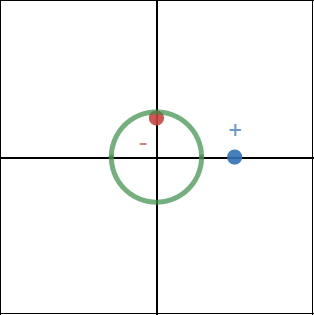
\includegraphics[width = 1.5in,height=1.5in]{shatter2-1}} 
				\subfloat[]{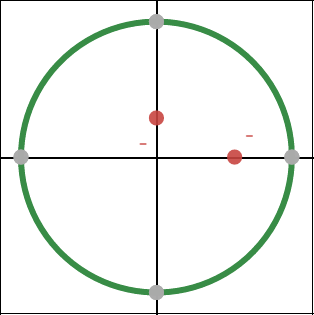
\includegraphics[width = 1.5in,height=1.5in]{shatter2-2}}\\
				\subfloat[]{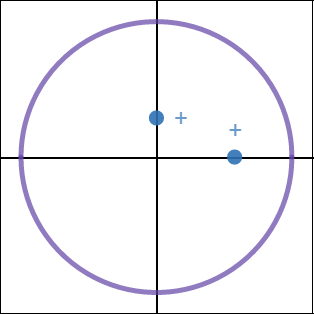
\includegraphics[width = 1.5in,height=1.5in]{shatter2-3}}
				\subfloat[]{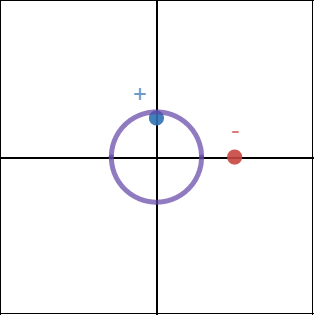
\includegraphics[width = 1.5in,height=1.5in]{shatter2-4}} \\
				\caption{Shattering 2 Points}
				\label{fig:shattering2}
			\end{figure}
		
			Now we need to show that there is no possible placement of three points that can be shattered. Let $\xb_1,\xb_2,\xb_3$ be the three points in $\R^2$. Then, let $r_1,r_2,r_3$ be the distance from the origin to $\xb_1,\xb_2,\xb_3$ respectively. Assume without loss of generality that $r_1 \leq r_2 \leq r_3$. Then, choose a labeling $\xb_1 = +, \xb_2 = -,$ and $\xb_3 = +$. To classify this correctly, we have two possibilities. First, we can have both $\xb_1$ and $\xb_3$ inside $H_{+,r}$ for some $r$. Choose $H_{+,r_3}$ which contains $\xb_1$ and $\xb_3$ as desired but also $\xb_2$ since $r_2 \leq r_3$. Therefore, this classifier does not achieve 100\% accuracy. Choosing any $r > r_3$ will not fix this problem. Our other choice is to choose some $r$ such that $\xb_2 \in H_{-,r}$. We let $r \geq r_2$ so $H_{-,r}$ contains $\xb_2$. However, it also contains $\xb_1$ since $r_1 \leq r_2$, Thus, this classifier fails to achieve 100\% accuracy. So, we have shown that there is no way to shatter 3 points with this family of classifiers. 
			
			\textit{EXTRA CREDIT (10 pts): Consider the class of hypotheses defined by circles anywhere in 2D
				space. A hypothesis h in this class will classify points as positive if they lie on the boundary or
				interior of the circle, and classify points as negative if they lie on the exterior of the circle. State
				and prove (rigorously) the VC dimension of this family of classifiers.}
			
				The VC dimension is 3. To show that we can shatter 3 points, choose the equilateral triangle with vertices $(-1,0), (1,0), (0,\sqrt{3})$. If all the labels are positive, then choose the circle $x^2 + y^2  = 4$ which contains this triangle since no point is further than $\sqrt{3}$ from the origin. If all the labels are negative, then choose the circle $x^2 + y^2 = \frac{1}{2}$ which contains no points of the triangle since every point is at least a distance of 1 from the origin. If only one of the vertices is positive, just choose a circle centered at the point with radius 1/2. This will only contain this single vertex since the distance between any two points is 2. The only hard case is if two of the vertices are positive. Then, the circle centered at the midpoint between the two points of radius 1 will contain both positive vertices on the boundary and not include the third point. For instance, if the points $(-1,0)$ and $(1,0)$ are positive, then the circle $x^2+y^2 = 1$ will classify the points correctly. By symmetry of an equilateral triangle, similar constructions will work for the other two pairs of points being positive as well.  
				
				To prove that it is impossible to shatter four points, we will break the problem into two cases. First, assume that the fourth point lies inside the convex hull created by the other three points. Label this interior point as $-$ and the other three points as $+$. Then, to classify this correctly, it would require having all three positive points inside a circle. However, the since the fourth point labeled with $-$ is inside the convex hull of the other three, it must also lie inside the circle so it cannot be classified correctly.
				
				The other case is where no point lies in the convex hull of the other three. Label the points $a,b,c,d$. Without loss of generality, assume that the largest distance between any two of these points is between $a$ and $c$ with a distance $d$. Label these points $a$ and $c$ as positive and label the points $b$ and $d$ as negative. Then two classify these points correctly, we would require a circle centered on the center of the line between $a$ and $c$ with radius $d/2$. Call this circle $A$. Then, the points $b$ and $d$ have to lie inside the circle. If one of them (assume it is $b$) was not inside the circle, then it would be a distance greater than $d/2$ from the center of $A$. This would mean that the the distance to $b$ from either $a$ or $c$ would be greater than $d$ which contradicts our assumption that $a$ and $c$ are the furthest points from each other. Thus, all four points must lie inside $A$ which means that we cannot classify all points correctly. This means that this family of classifiers cannot shatter 4 points. Thus, the VC dimension is 3. 
	\end{solution*}
\end{document}